%Hello test

\documentclass[jou,a4paper,notxfonts]{apa}
\usepackage{graphicx} 
\usepackage{palatino}
\usepackage{fancyhdr}
\usepackage{url}
\pagestyle{fancy}




% header on first page
\fancypagestyle{plain}{%
\fancyhf{} % clear all header and footer fields
\fancyhead[L]{\small
ECEM 2013 Proceedings}
\fancyfoot[C]{\thepage}
\renewcommand{\headrulewidth}{0pt}
\renewcommand{\footrulewidth}{0pt}}

\title{Interacting with Objects in the Environment by Gaze and Hand Gestures}

%please refer to http://www.ilsp.gr/homepages/protopapas/apacls.html#titlhead for different numbers of authors and affiliations
\threeauthors{Jeremy Hales}{David Rozado}{Diako Mardanbegi}
\threeaffiliations{ICT Centre - CSIRO}{ICT Centre - CSIRO}{ITU Copenhagen}

\journal{}
\volume{}
%Guys keep in mind the abstract can not be longer than 200 words!
\abstract{ A head-mounted wireless gaze tracker in the form of gaze tracking glasses is used here for continuous and mobile
monitoring of a subject's point of regard on the surrounding environment. We combine gaze tracking and hand gesture recognition to allow a subject to interact with objects in the environment by gazing at them, and controlling the object
using hand gesture commands. The gaze tracking glasses was made from low-cost hardware consisting of a safety glasses' frame and
wireless eye tracking and scene cameras. An open source gaze estimation algorithm is used for eye tracking and user's
gaze estimation. A visual markers recognition library is used to identify objects in the environment through the scene
camera. A hand gesture classification algorithm is used to recognize hand-based control commands. When combining all
these elements the emerging system permits a subject to move freely in an environment, select the object he wants to
interact with using gaze (identification) and transmit a command to it by performing a hand gesture (control). The
system identifies the target for interaction by using visual markers. This innovative HCI paradigm opens up new forms of
interaction with objects in smart environments.
\linebreak \linebreak {\bf Keywords: Eye Tracking, Gaze Tracking, Head-Mounted Gaze Tracker, Eye Tracking Glasses, Mobile Interaction, Hand Gestures, Gaze Interaction, HCI, Gaze Aware Systems, Gaze Responsive Interface, Mobile Interaction}}

\acknowledgements{This paper has been possible thanks to the CSIRO ICT Centre Undergraduate Vacation Scholarships Program. Corresponding author: jeremy.hales1@gmail.com}
\shorttitle{Interacting with Objects in the Environment by Gaze and Hand Gestures}
\rightheader{}

% repeat the authors here (use et al if more than three authors):
\leftheader{ }

\begin{document}
\maketitle

\lhead{\small
ECEM 2013 Proceedings\\
}
\rhead{
Hales, J., Rozado, D., \& Mardanbegi, D. (2013)\\
Interacting with the Environment by Gaze and Hand Gestures
}
\thispagestyle{plain}

\section{Introduction} 
% We should clearify that this paper does not contribute in the hand gesture recognition but it uses the gesture and
% gaze in a mobile situation for controlling a robot.
Body language and gaze are important forms of communication among humans. In this work, we present a system that
combines gaze pointing and hand gestures to interact with objects in the environment. Our system merges a video-based gaze
tracker, a hand gesture classifier and a visual marker recognition module into an innovate HCI device that permits novel
forms of interaction with electronic devices in the environment. Gaze is used as a pointing mechanism to select the
object which the subject wants to interact with. A visual binary marker attached to the object is used for
identification of the object by the system. Finally, a hand gesture is mapped to a specific control command that makes
the object being gazed at to carry out a particular function.

Using gaze for interaction with computers was initiated in the early 1980s \cite{bolt1982eyes} and further developed by \cite{ware1987evaluation}. Today, gaze interaction is mostly done using a remote eye tracker with a single user sitting in front of a
computer display. However, head-mounted gaze trackers (HMGT) allow for a higher degree of mobility and flexibility,
where the eye tracker is mounted on the user and thus allows gaze to be estimated when e.g. walking and driving. HMGT
systems are commonly used for estimating the gaze point of the user in his field of view. However, the point of regard
(PoR) obtained by head-mounted gaze trackers can be used for interaction with many different types of objects present in  the environments during our daily activities. There has been some previous work done on using gaze for interaction with computers in
mobile scenarios using head-mounted gaze trackers \cite{Mardanbegi2011}. Despite the fact that gaze can be used as a mechanism for pointing in many interactive applications, eye information has been shown to be limited for interaction purposes.
The PoR can be used for pointing, but not for yielding any additional commands. The main reason is that it is unnatural
to overload a perceptual channel such as vision with a motor control task \cite{magicPointing}.
Therefore, other interaction modalities such as body gestures and speech together with gaze can be used for enhancing
gaze-based interaction with computers and also with electronic objects in the environment.  In this paper, we use
hand gestures to circumvent the limitations of gaze to convey control commands. The combination of gaze and hand
gestures enhances the interaction possibilities in a fully mobile scenario.
 
 Automatic gesture recognition is a topic in computer science and language technology that strives to interpret human
 gestures via computational algorithms. Gestures can originate from any bodily motion or state but commonly originate
 from the face or the hands. An appealing feature of gestural interfaces is that they make it possible for users to
 communicate with objects without the need for external control devices. Hand gestures are an obvious choice as a
 mechanism to interact with objects in the environment. Automated hand gesture
 recognition is challenging since in order for such an approach to represent a serious alternative to conventional input
 devices, applications based on computer vision should be able to work successfully under uncontrolled light conditions,
 backgrounds and perspectives. In addition, deformable and articulated objects like hands represent added difficulty
 both for segmentation and shape recognition purposes. This paper does not intent to contribute significantly in the topic of hand gesture recognition methodology, but rather to suggest the combination of gaze and hand gestures as an alternative to the conventional methods that are used for  gaze interaction such as: blinking (e.g., \cite{mackenzie2008eye}), dwelling (e.g., \cite{jacob_use_1991}), and gaze gestures (e.g., \cite{isokoski2000text}). We use the scene image of the HMGT system for recognizing the hand gestures and for recognizing the
 visual markers attached to the gazed objects. The hand gesture recognition module we developed here is able to detect a
 hand in front of the scene camera of the HMGT and the number of fingers that the hand is holding up as well as its relative movements in 4 spatial directions.
 
 In summary, this work represents a proof of concept for an innovative form of interacting with objects in the
 environment by combining gaze and hand gestures. Interaction is achieved by gazing at an object in the environment and
 carrying out a hand gesture. The hand gesture specifies a certain command and gazing at the object, and the visual
 marker associated to it, make only that specific object to respond to the subsequent hand gesture. The low cost off-the-shelf
 components used to build the hardware, and the open source nature of the algorithms used for gaze estimation and object recognition, make this form of interaction amenable for spreading among academic institutions and research labs to further investigate and stretch the possibilities of this innovative HCI paradigm.

The remaining of the paper is structured as follows. The \emph{Related Work} section provides an overview of the literature on the topic of gaze and mobile interaction. The \emph{System Overview} section delineates the main components of the system and their mutual interactions. The \emph{Implementation} Section goes into a detailed description of each of the system's components. The \emph{Application Example} Section describes a particular instantiation of our system to control 3 objects in an environment: an Arduino board, a computer and a robot. Finally, the \emph{Discussion and Conclusion} Section elaborates in some of the issues we have found when trying out the proposed gaze and hand gestures based interaction as well as pointing out possible future research venues to continue exploring the innovative interaction modality proposed here.


% Diako: <the following paragraph about the eye tracking should be removed> Eye tracking refers to the monitoring of eye
% movements. Gaze tracking is the process of measuring the point of regard (where a person is looking). A head mounted
% eye tracker is a device that permits measuring eye movement while the subject is moving around an environment and
% estimate the position of gaze in the environment. Eye trackers are used in research on the visual system, in
% psychology, in cognitive linguistics, product design and in Human Computer Interaction (HCI) research
% \cite{myiwann2011}. There are a number of methods for measuring eye movement. The most popular variant uses video
% images from which the eye position is extracted. Other methods use search coils or are based on electrooculography.




\section{Related Work}
%Diako! My subsections are only a suggestion. you know better than me how to properly organize this section :)


%\subsection{Hand gestures in HCI}
%-------hand gesture
 There has been substantial research in hand/body gestures used for human-computer interaction. There are many vision-based methods that by using video cameras as the input device, can detect, track and recognize hand gestures with various image features and hand models \cite{surveygesturerecognition}. Most of these approaches detect and segment the hand in the image using the skin color information \cite{argyros2004real}. In this paper we have used a color based hand gesture recognition method that is efficient and easy to implement.
%-------hand gesture in HCI
 Hand gestures can be used as a mode of HCI that can simply enhance the human-computer interaction by making it more natural and intuitive. Some of the application domains where gestural interfaces have been comonly used is in virtual environments (VEs) (\cite{adam1993virtual, krueger1991artificial}), augmented reality \cite{buchmann2004fingartips} and automatic sign language recognition \cite{Rozado2012b,myicann2010} in which hand gestures are comonly used for manipulating the virtual objects (VOs) for interaction with the display or for recognition of sign language.
%-------wearable hand gesture
The vision based hand gesture recognition devices can be worn by the user, providing the user with more flexibility and mobility for interaction with the environment \cite{starner2000gesture,amento2002sound}.

%------gaze gestures
More recently several authors have also investigated using gaze itself to generate gestures for control and interaction purposes \cite{istance, Rozado2012a, drewessecurity, myiwann2011, emilieetra, interactingWithComputerUsingGazeGestures}. While useful in many regards, by being very fast to perform and robust under low gaze estimation accuracy, gaze gestures also possess shortfalls in terms of risking to overload the visual channel which is intuitively perceived by users as just an input channel.
%-------Multimodal

There is also a body of literature focused around gestures for multimodal interactions \cite{starner2000gesture,schapira2001experimental,nickel2003pointing,Rozado2012}. For example, hand gestures in combination with speech provide a multimodal interactions mechanism that allows the user to have an eyes-free interaction with the environment. Body gestures can also be combined with gaze in situations where the gazed context is the interaction object (e.g., looking at a lamp and turning the lamp on). In such cases, gaze acts as a complementary interaction modality and it is used for pointing. \cite{mardanbegi2012eye} used head gestures together with gaze for controlling objects in the environment by gazing at the objects and then performing a head gesture. Authors used a mobile gaze tracker for gaze estimation and an eye-based method for measuring the relative head movements. They used the scene image for recognizing the objects and to ensure that the PoR is on the object during the gesture. In contrast, in this paper, we use gaze for pointing and hand gestures to execute a particular command using the scene camera of a head-mounted eye tracker for measuring the hand gestures, see Figure \ref{Method}.


\begin{figure}[tp]
 \includegraphics[width=0.5 \textwidth]{Method.jpeg}
 \caption{\textbf{Overview of the interaction modality proposed in this work.} The diagram describes the main components and actions involved in interacting with objects through gaze and hand gestures.}
 % the label is used to put refrences to this figure in the text
 \label{Method}
\end{figure}

 
%How to insert a figure (image):
\begin{figure}[tp]
 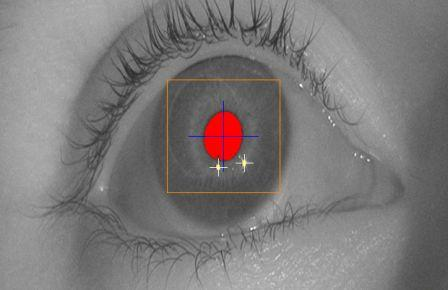
\includegraphics[width=0.5 \textwidth]{screenGazeTracker.jpg}
 \caption{\textbf{The Open Source Haytham Gaze Tracker Tracking the Eye.} The
features tracked in the image are the pupil center and two corneal reflections. These features are 
used by the gaze estimation algorithms to determine the PoR of the user on the scene camera.}
 % the label is used to put refrences to this figure in the text
 \label{screenGazeTracker}
\end{figure}

\section{System Overview}

%Do not go to the details and implementation please. Only general talk and method. 

%-------- Method in general (gaze + gesture + interaction)
In this section, different steps of the interaction process are introduced and the main elements of the system are described. 
In our system, a head-mounted gaze tracker estimates the gaze point in the user's field of view using an eye tracking camera and an scene camera. A simple method for recognizing the objects in the environment is used by detecting visual markers associated to them through the scene camera. When the subject carrying the gaze tracker looks at an object, the visual marker placed on the object is recognized by the system. When a visual marker has been detected, the hand gesture recognition algorithm will be activated in the scene image (for a short period of time) to detect the potential hand gesture that might be generated shortly after. A control command, associated to a specific hand gesture, will be send to the object if the gesture is detected. In this way, only that particular object in the environment gazed at will react to the hand gesture, while the rest of the objects in the environment susceptible to be controlled by gaze remain unresponsive.

%good Sketch of the method here
The main hardware components of the system are introduced below:
\begin{enumerate}
\item[a)] A wireless mobile gaze tracker glasses with two cameras: one for tracking one eye and the other to capture the field of view of the subject. 
\item[b)] Video receiver that is connected to a remote PC and receives the video streams of both the eye and the scene camera.
\item[c)] Visual markers attached to the target objects of interaction. 
\item[d)] Interaction objects (e.g, robot, lamp, computer display).

\end{enumerate}

The processing units of the system can be conceptually divided into two groups: the server and the clients, see Figure \ref{systemDiagram}. The server processes the eye and the scene images. Eye tracking, gaze estimation, and recognizing the visual markers and the hand gestures are done in the server application running on a remote PC. The output of the application will be sent to the client application controling a specific object using the TCP/IP protocol. The client applications facilitates the connection between the server and the objects in the environment and undergoes the local processing needed for controlling the objects. 

\begin{figure}[tp]
 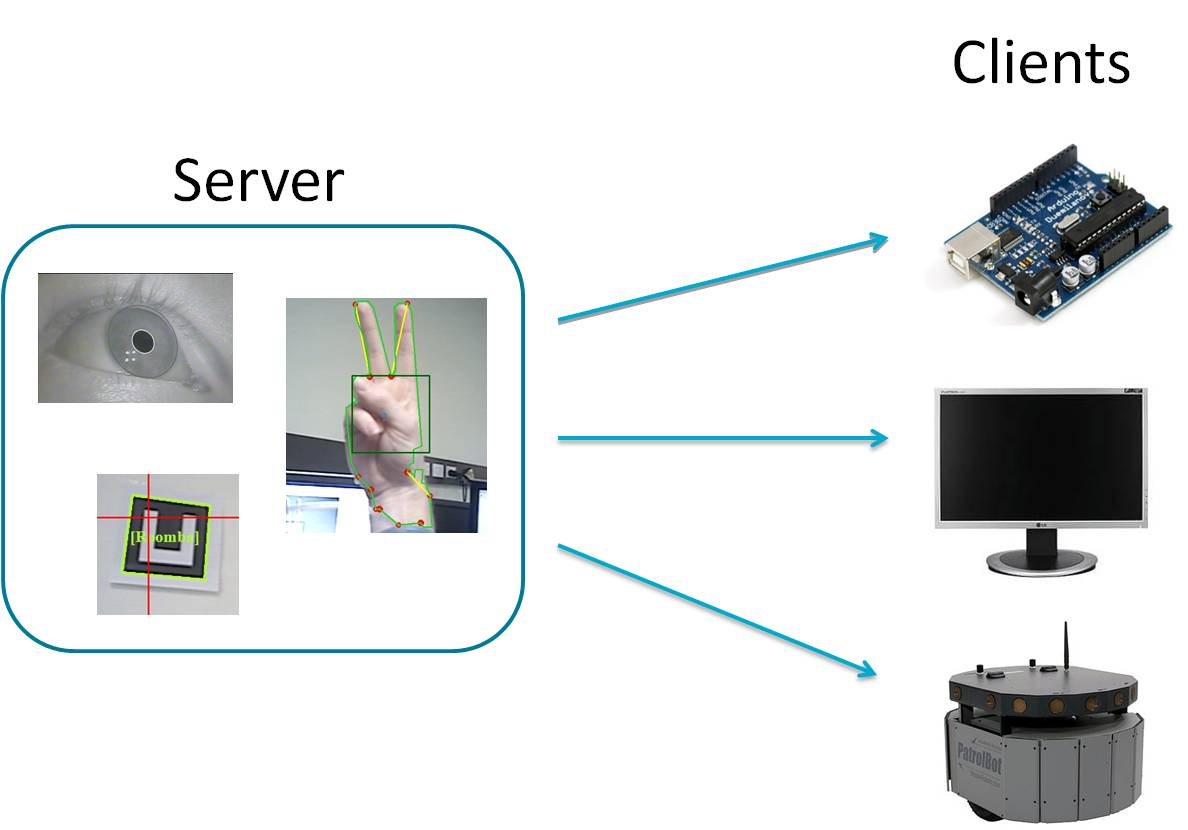
\includegraphics[width=0.5 \textwidth]{systemDiagram.jpg}
 \caption{\textbf{System Diagram.} Several smart objects \emph{clients} connect to a centralized servers that handles the gaze tracking and estimation, the visual marker recognition and the hand gesture recognition. The server dispatches the appropriate commands to a given client when a combination of gaze fixation on the object visual marker and hand gesture is detected.}
 % the label is used to put refrences to this figure in the text
 \label{systemDiagram}
\end{figure}


\paragraph{Gaze Tracking}
%Eyes are used by humans to obtain information about the surroundings and to communicate information. When something attracts our attention, we position our gaze on it, thus performing a \textit{fixation}. A fixation usually has a duration of at least 150 milliseconds (ms). The fast eye movements that occur between fixations are known as\textit{saccades}, and they are used to reposition the eye so that the object of interest is projected onto the fovea. The direction of gaze thus reflects the focus of \textit{attention} and also provides an indirect hint for \textit{intention} \cite{velichkovsky}.


Depending on the hardware configuration of the different components, gaze tracking systems can be classified as either \textit{remote} or \textit{head-mounted}. In remote systems, the camera and the light sources are detached from the
user and normally located around the device's screen, whereas in head-mounted systems the components are attached to the user's head. Head-mounted eye trackers can be used for mobile gaze estimation as well as gaze interaction purposes. The head-mounted gaze trackers have two cameras: one for recording the eye image and one for recording the scene image. In this work, we have used a head-mounted gaze tracker for gaze estimation on top of which, we have build a hand gesture recognition module. The point of regard and the coordinates of the gaze point in the scene image are measured by the system.  

\paragraph{Object recognition}
Visual markers provide a simple solution for recognizing the objects in the scene allowing us to concentrate on illustrating the potential of the proposed interaction method. Visual marker recognition systems consist of a set of patterns that can be detected by a computer equipped with a camera and an appropriate detection algorithm \cite{middel19detection}. Markers placed in the environment provide easily detectable visual cues that can be associated to specific objects for identification purposes. Once a visual marker is recognized in the vicinity of the user's gaze, the hand gesture recognition algorithm will be activated.

\paragraph{Hand Gesture}
A skin color-based method is used for detecting the hand in the scene image. The hand gesture recognition worked well for natural skin color, but using a latex glove of a color not present in the environment improves the performance. Hand gestures are defined as holding the hand with a preset number of fingers for a predefined dwell time of 1 second (a static hand gesture) and moving it in a particular direction (a dynamic hand gesture): up, down, left  or right. Therefore, the hand recognition part consists of two steps: detecting a static shape of the hand and then a dynamic hand gesture that ends by taking the hand outside the image.
 
The gesture alphabet can be named using a combination of the number of fingers held up, x, and one of the four spatial directions that the hand is supposed to move to generate the gesture, D, in a pattern such as xD. For example 4Up, refers to a gesture consisting of the hand holding four fingers up and an upwards movement.
%-------------------------------------------------

\section{Implementation}

The presented method has been implemented in a real scenario for controlling a remote robot, an Arduino, and a computer display. In this section, implementation and the hardware/software components of the system are introduced briefly. 

\subsection{Gaze Tracking System}

\begin{figure}[tp]
 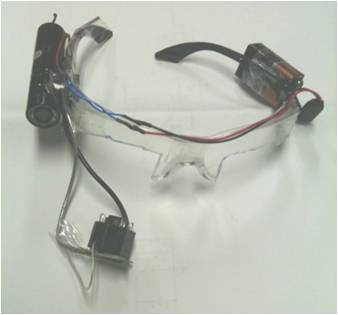
\includegraphics[width=0.5 \textwidth]{gazeTrackingGlasses.jpg}
 \caption{\textbf{Low Cost Gaze Tracking Glasses.} The wireless camera on the top left of the figure is what we refer to in this work as the scene camera. The scene camera approximately captures the field of view of the user. The camera on the bottom left of the figure is the gaze tracking camera that monitors the user's gaze movements. The Haytham software uses the video stream provided by that eye camera to calculate the PoR of the user and superimposes the gaze estimation coordinates over the  video stream generated by the scene camera. The top right of the figure shows the battery that is used to provide energy to the wireless cameras.}
 \label{gazeTrackingGlasses}
\end{figure}

\begin{figure}[tp]
 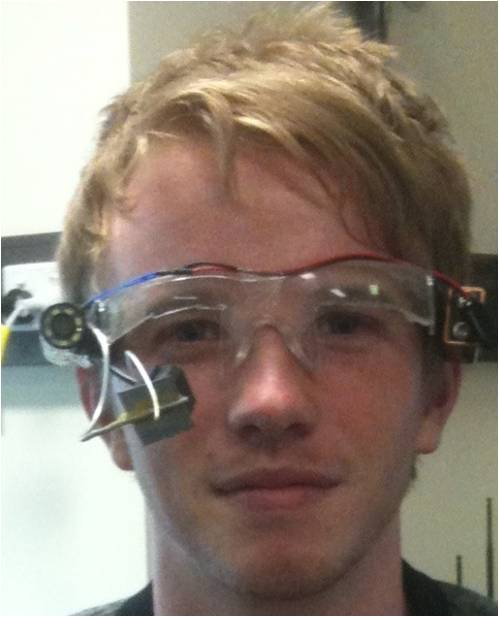
\includegraphics[width=0.5 \textwidth]{jeremy.jpg}
 \caption{\textbf{Low Cost Gaze Tracking Glasses On a Subject.} This figure shows how the low-cost head-mounted gaze
 tracking system looks while being used by a subject.}
 \label{jeremy}
\end{figure}

We have build a low-cost head-mounted gaze tracker using off-the-shelf components (Figure \ref{gazeTrackingGlasses} and Figure \ref{jeremy}). The system consists of
safety glasses, batteries, and the wireless eye/scene cameras. The wireless eye camera
is equipped with infrared emitting diodes that permit the gaze tracking software to monitor the position of the pupil and the glint in the image. These features are used by the gaze estimation algorithm to estimate the PoR. Infrared light improves image contrast and produces a reflection on
the cornea, known as corneal reflection or glint. A calibration procedure needs to be done to build a user specific model of the eye. The calibration procedure consists on the user looking at a number of points on the environment and marking them on the scene image while the user fixates on them. Once the calibration procedure is completed, the gaze estimation algorithm is able to determine the point of regard of the user in the environment. Figure \ref{screenGazeTracker} shows a screenshot of an eye being tracked by the open source gaze tracker  \cite{mardanbegi2012eye} used in this work. In the figure, the center of the pupil and two corneal reflections are the features being tracked.

\subsubsection{Making the head-mounted eye tracker glasses}\hspace{0pt} \\

Figure \ref{gazeTrackingGlasses} shows a prototype of the eye tracking glasses built for this work. An area was traced onto the lens of a pair of safety glasses where the eyes will be approximately located when the user puts on the glasses. Tin snips were used to cut away the plastic parts of the lenses bounded by the previously traced areas. It is important that the majority of the lenses of the glasses is left intact to preserve the structural integrity of the frame. Tin was cut to the size and shape of the infrared camera using the tin snips. Steel wire was used to attach the camera to the frame of the glasses. The wire was cut to a size of 25cm and attached to the piece of tin using araldite. Double sided tape was used to secure the tin to the back of the camera. The wire was bent into an 'L' shape and firmly attached to the right hand side of the glasses (frame) using tape. The infrared camera runs on a 9V battery that also needed to be mounted to the glasses. The connecting wires from the battery to the camera were extended and the battery was attached to the left hand side of the glasses. This distributes the weight of the components over the frame. Utilising the Haytham software, the position of the camera was checked to ensure the camera was capturing the entire eye. It was found that the best position of the eye camera is below the glasses so it doesn't obstruct the user's vision. The scene camera was firmly mounted to the right side of the glasses using tape as close as possible to the eye in order to minimize the parallax error, see Figure \ref{jeremy}.

\subsubsection{Gaze tracking software}\hspace{0pt} \\
We used the Haytham\footnote{\url{http://itu.dk/research/eye/}} open source gaze tracker to monitor user's gaze. The Haytham gaze tracker provides real-time gaze estimation in the scene image as well as visual marker recognition in the scene camera video stream. Figure \ref{visualMarker} shows a recognized marker from the scene video stream and the gaze point measured by the gaze tracker represented as a cross hair. 

\subsection{Implementing hand gestures recognition}

\begin{figure}[tp]
 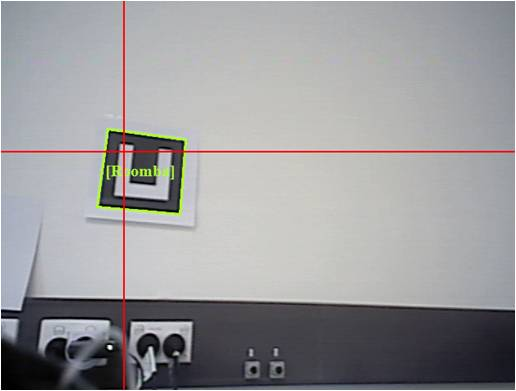
\includegraphics[width=0.5 \textwidth]{visualMarker.jpg}
 \caption{\textbf{Visual Marker Recognition.} The Hayhtham gaze tracker uses the Aforge glyph processing library (GRATF) for visual marker recognition in the scene image. This figure shows the identified marker and the user's gaze point (cross hair) in the scene image. When a subject position  its gaze  on a visual marker that identifies an object, the system interprets this as a pointing action and sends the subsequent recognized hand gestures to the  specific object represented by the visual marker.}
 % the label is used to put refrences to this figure in the text
 \label{visualMarker}
\end{figure}

\begin{figure}[tp]
 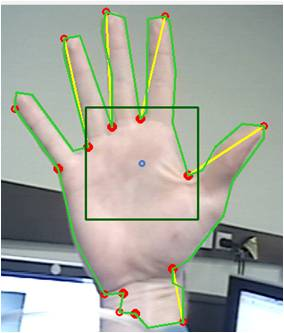
\includegraphics[width=0.5 \textwidth]{hand.jpg}
 \caption{\textbf{Hand Pose Recognition Through the Scene Camera.} The figure shows a hand with five fingers held 
 up as recognized through the scene camera by the hand pose recognition routine. The light green line outlines the convex hull of the hand and the dark green box represents the boundary for a classified movement.}
 % the label is used to put refrences to this figure in the text
 \label{hand}
\end{figure}

\subsubsection{Static hand gesture recognition algorithm}\hspace{0pt} \\
An open source hand gesture recognition software\footnote{\url{http://blogs.ugidotnet.org/wetblog/Default.aspx}} developed by Luca Del Tongo was modified for use in detecting the number of fingers raised by the hand. There are two options for analysing the images captured by the scene camera: colour or skin detection. To detect the skin of the hand the image was transformed to the Ycc colour space; upper and lower bounds were set for the Cr and Cb channels. To detect a coloured latex glove, the image was transformed to the HSV colour space; upper and lower bounds were set for the hue and saturation channels. Pixels that satisfied the bounding conditions are identified as potential sections of the hand. Two measures were implemented to reduce false detection caused by noise or objects with similar colours to skin or the coloured gloves. The blob with the largest contour area is designated as the hand and all blobs that are lower than a set area are removed from the image, including the blob that has been designated as the hand. This removes the possibility that small blobs (noise) are identified as the hand of the user. The convex hull is extracted from the hand and the convexity defects are determined (Figure \ref{hand}). Two parameters of the defects were used; the start and the end points are the points on the hull that mark where the defect starts and end. Three conditions were defined to determine whether a defect is a raised finger. They are: the start point of a defect must be higher than the end point, either the start or end points must be higher than the centre of the hand and the magnitude of the start and end points must be greater than the scaled down length of the hand. Each defect is checked and the total number of fingers identified is the sum of defects that satisfy the aforementioned conditions. 

\subsubsection{Dynamic hand gesture recognition algorithm}\hspace{0pt} \\
The centroid of the hand contour is determined and an initial boundary box of size 20x20 pixels set. If the centroid doesn't move outside of the boundary box for 1.5 seconds, the current position of the hand is identified as the reference point and a new boundary box of size 60x60 pixels is set. If the centroid of the hand moves outside of the box it is classified as a movement. The location of the centroid when it moves outside the box designated the direction of movement: above the box is up, below the box is down, left of the box is left and right of the box is right. The program samples and averages the number of fingers shown. This helps to eliminate false identification of the number of fingers due to noise. When a movement is identified, the average number of fingers is sent to the client with the direction of movement.

\subsection{Clients}
A client program was developed to communicate with the devices in the environment. The program connects to the server (Haytham) using the TCP/IP protocol. Haytham sends commands to the client detailing specifics such as: the marker that has been recognised, the number of fingers raised and the direction of movement of the hand. 

The proposed method is used for controlling a patrol robot, controlling an Arduino, and for interaction with a computer display (Figure \ref{systemDiagram}) as described below.

The patrol robot connects to the computer using an Ethernet cable. The number of fingers determines the magnitude of movement and the hand movement controls the direction of movement (e.g. 2Up will move the robot forward with a magnitude of 2 and 3Left will rotate the robot counter-clockwise). An Arduino is connected to the client program via serial connection and is used to control 3 leds on a breadboard. The interaction with the computer display is done by minimizing or maximizing the windows in the display through use of the sendMessage function.
%I don't think the next lines are neccessary here since we say the same in the application section, and that is a section where we have little "meat" to show, so I would rather 
%The hand movement 2Up turns on all the leds and 4Left turns them all off.
%The hand movement 2Up minimises all applications open and 4Left reminimises them all.

\begin{figure}[tp]
 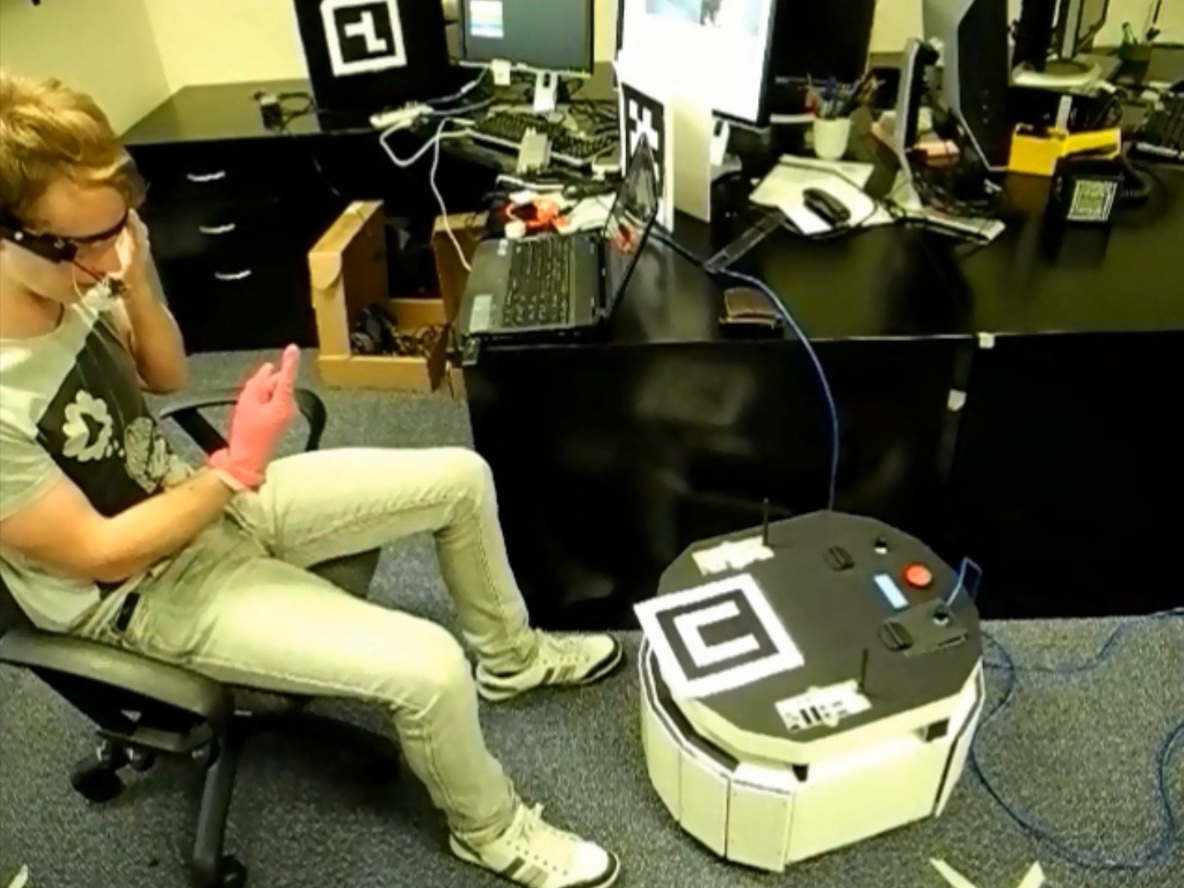
\includegraphics[width=0.5 \textwidth]{systemAtWork.jpg}
 \caption{\textbf{System At Work.} This figure shows the user gazing at the visual marker, identifying the robot. A hand gesture is performed to transmit a movement command to the robot.}
 % the label is used to put refrences to this figure in the text
 \label{systemAtWork}
\end{figure}

\section{Application Example}
% Diako, I was wondering if we can really refer to our trials with the system as a ``pilot study''. What do you think?
We carried out a small pilot study to test the functionality and performance of the system. We decided to test the
system in a environment where 3 ``smart'' objects could be controlled by the system simultaneously: a computer, a set of
leds in a breadboard and a robot. The hand gesture recognition module could recognize 5 different states of the hands
as defined by the number of fingers being held up: 1, 2, 3, 4 and 5. A gesture was defined as one of these 5 states plus
one of four spatial directions: up, down, left and right.

The breadboard responded to users commands just by turning the infrared leds on and off. Two fingers being held up and
an upward movement would turn the leds on. Four fingers being held up and a movement to the right would turn them off.

The same hand gestures were used to control the computer. The upward movement of the hand with two fingers being held up
was mapped to a command in the operating system that minimizes all the current open windows on display in the computer
GUI. Four fingers being hold up and a movement to the right gesture was mapped to a command that brings all the
minimized windows back up. This particular set of gestures and control commands were not selected specifically for
any particular reason other than as a proof of concept. Any other type of gestures associated to different
control commands could be envisioned and implemented.

The robotic control example was the most elaborated one. The robot could be made to move forward or backward and to turn right or
left. The numbers of fingers being held up with the hand indicated, either the speed for forward and backward movements
or the amount of turn to be made for right and left movements.

The hand gestures could be done with bare hands, but we noticed that in environments where the color of the walls could
resemble the skin hue, hand gesture recognition performance would suffer. Using a glove with a distinctive color, not 
present in the rest of the environment, enhanced hand recognition performance.

This manuscript's associated video\footnote{\url{http://youtu.be/SGqF1Mi6JGI}} provides a good visual overview of the system at work and how it is being used by two different users to interact with a computer, a breadboard
with a set of light emitting diodes and with a robot.


% ---------------------------------------------------------------
\section{Discussion and Conclusion}
In this work we have shown how to interact with objects in the environment through an innovative combination of gaze and
hand gestures using a set of gaze tracking glasses and a hand gesture recognition module. The method is easily
extensible to multiple objects in the environment and to a wide array of hand gestures.

The low-cost head-mounted eye tracker used and the gaze estimation algorithms employed do not compensate for parallax
error, i.e. the inability to differentiate between the working plane and the calibration plane
\cite{mardanbegi2012parallax}. This limits the ability to alternate interaction with objects at a distance and objects
up close. Nonetheless, since the scene camera used in the glasses is relatively close to the eye being tracked, see Figure
\ref{gazeTrackingGlasses}, the parallax error was minimized. Furthermore, we noticed that during the calibration, using                                                                                                                                                                                                                                                                                                                                                                                                                                 
calibration points situated at different distances (from 1 to 10 meters) would achieve a compromise between objects
far away and objects up close and would generate good gaze estimation for all sort of distances. We noticed that
gaze estimation accuracy was never an issue for our system. Only over time, if the glasses would move slightly from
their position during calibration, due to sweat on the skin or drastic head movements that would cause the glasses to slide slightly, would gaze estimation degrade marginally.


We did notice problems with the skin detection algorithms when the hand was position within the field of view of the
scene camera. This was markedly noticeable, when the colors of the background were similar to the skin color. Usage of
more sophisticated skin detection algorithms could help to solve this issue.


An important issue of the system was the fact that the user wearing the glasses did not have any sort of feedback signal in
terms of where within the field of view of the scene camera the hand was placed when it was about to initiate a hand
gesture. This was due to the lack of a display on the glasses to provided visual feedback in terms of how the hand is
positioned within the field of view of the scene camera. We implemented an auditory feedback signal to indicate
that the system had found the hand holding a number of fingers up within the field of view of the scene camera and it was therefore ready to receive a
gesture. We found that this helped the user but still did not provide real time feedback to carry out small
corrections of hand positioning for proper positioning within the field of view of the scene camera. This issue was due
to the usage of a scene camera with a relatively narrow field of view. Using a scene camera with a wider field of view
should prevent the need of feedback for hand positioning with high granularity precision since the hand would always fall within the field of view of the scene camera as long as the arm was stretched in front of the user.
 

Further work should strive to carry out an extensive quantitative analysis of the performance of the system within a
large user study and in comparison to alternative modalities of gestures based interaction with objects in the environment through gaze alone, gaze and voice, and gaze and head gestures. 


More sophisticated hand gestures that the ones described here can also be envisioned. However, complex gaze gestures generate a
cognitive and physiological load on the user. Cognitively it is difficult for users to remember a large set of complex
gestures, and physiologically it is tiring and challenging to complete them. Finding the right trade-off between simple
and complex hand gestures is therefore paramount to successfully use hand gestures as a control input device.

More reliable hand tracking technologies that use depth sensor such as  infrared laser projections to be combined with monochrome CMOS sensor, able to capture video data in 3D under any ambient light conditions, would greatly enhance the robustness of the hand recognition algorithms, making our system as a whole more reliable.


The preliminary results obtained  in this pilot work shows promise for this form of interaction with objects in the
environment. The combination of gaze and hand gestures to select an object  and emit a control command are both natural 
to potential users and fast to carry out liberating users of the need to carry control devices in their hands. The richness of hand gestures potentially available suggests that this form of interaction can be used for sophisticated and complex environments requiring  a large set of control commands while allowing the user to remain mobile in the environment.




%assumes that there is a biblio.bib file in the same directory
\bibliography{library}
\end{document}

